\section{Background}
\label{sectbackground} 

This section overviews the structure of a modern JS runtime. It also
provides a concise description of the components that are used by \natisand
to build the sandbox.

\vspace{-0.52em}
\subsection{JS runtimes}
\label{sect:background-js-runtime}

JS code rendering is a complex process, involving tasks such as code
compilation, code optimization, memory allocation, runtime garbage
collection of objects no longer needed, and many others. To perform
these critical tasks, modern JS runtimes rely on {\em engines},
dedicated components implementing the ECMAScript specification that
were originally developed for web browsers. As already mentioned in
Section~\ref{sect:introduction}, Node.js and Deno embed Google's
V8~\cite{v8-site}, while Bun relies on
JavaScriptCore~\cite{javascriptcore}. The interoperability between
runtime and engine is achieved with specialized bindings, which are
defined in the {\em node:v8}~\cite{node-v8-bindings} module in the
case of Node.js, in the {\em rusty\textunderscore v8}~\cite{rusty-v8}
library for Deno, and by {\em webcore}~\cite{webcore-bindings} in Bun.

While an engine provides all the tools to securely execute JS code in
an isolated context (we call it the {\em JS context}), a development
platform requires complementary features to be fully functional. For
instance, a backend web application may need to open network
connections, handle several concurrent HTTP requests, or access the
filesystem to read configuration files. To address these requirements,
the architecture of a modern runtime extends the engine with various
runtime-specific components dedicated to the interaction with the host
system. A few well-known functions implemented following this design
pattern are: interaction with the filesystem (e.g., fs, Deno.FsFile),
creation of UNIX sockets (e.g., net), and exposure of HTTP servers
(e.g., http, Deno.serveHttp).

From the web application perspective there is no difference between
the functions defined by the ECMAScript standard, and the ones
provided by the runtime (and its
extensions)~\cite{brown2017finding,dinh2021favocado}.  However,
non-standard APIs are not served directly by the engine, but are
redirected to the runtime leveraging the aforementioned
bindings. Since these APIs deliberately permit to break the isolation
between the environment controlled by the engine and the underlying
system, JS runtimes allow developers to restrict them through the
definition of permissions~\cite{node-permissions,
  deno-permissions}. Based on the runtime, permissions work with
different granularities (e.g., single API vs set of APIs) and
different default behavior. For example, Deno uses a default-deny
model requiring the developer's explicit consent to access
system resources, with effect on multiple
APIs~\cite{deno-permissions}.

Permissions are intuitive and effective, but they do not offer
significant security guarantees when a module needs to run binary
programs, or import shared libraries to leverage cross-language
function calls~\cite{deno-permissions}. To do so, the web application
must be granted the permissions to call APIs like {\em command} or
{\em dlopen} (e.g., with {\tt allow-run} and {\tt allow-ffi}
flags in Deno). In the case of {\em dlopen}, native code is directly
copied into one of the processes owned by the runtime itself before
being executed, while with {\em command}, the runtime first delegates
to the OS the creation of a process with the {\tt clone} system call,
then performs an {\tt exec} to replace the process image and run the
desired program.  Independently of the runtime used, both APIs require
to execute code outside of the isolated context managed by the engine,
as shown in Figure~\ref{fig:js_runtime}, which means that this code
runs with the same privileges of the user executing the entire JS
application.

\begin{figure}[t]
  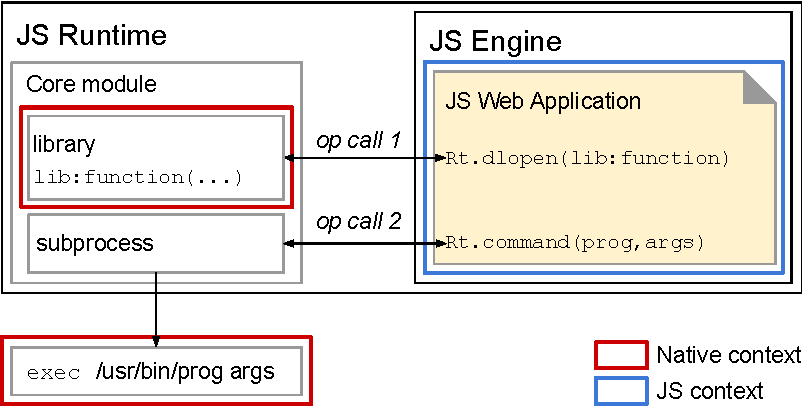
\includegraphics[width=\columnwidth]{chapters/natisand/fig/js_runtime}
  \caption[Execution of binary programs and shared libraries by JS
    runtimes]{
    Execution of binary programs and shared library functions by the
    JS runtime
  }
  \label{fig:js_runtime}
\end{figure}


\subsection{Components for resource protection}
\label{sect:background-sandboxing}

\subsubsection*{Landlock}

Landlock~\cite{landlock} is a Linux Security Module (LSM) introduced
in the kernel starting from release 5.13. The goal of Landlock is to
enable unprivileged applications to restrict their ambient rights in
accordance with the least privilege principle. Ambient rights are
specified by {\em rulesets} -- i.e., simple structures that
associate a set of permissible actions with a filesystem path (e.g.,
{\tt read} and {\tt exec} over the resources stored in {\tt
  /tmp}). Several rulesets can be combined to determine the final set
of actions available to an application. To make them effective, a call
to the {\tt landlock\textunderscore restrict\textunderscore self()}
function is performed.

The ambient rights granted by Landlock are thread-based, and are
automatically inherited by all the children subsequently created via
{\tt clone}. After a Landlock sandbox is enforced (either by self
restriction or inheritance), it is only possible to further narrow it.
It is also important to mention that Landlock is stackable, hence it
is fully composable with other LSMs already available on the host, such
as SELinux, AppArmor and SMACK.
%
Although Landlock offers a simple, yet powerful, sandboxing API,
currently, the protection offered is only limited to the filesystem.


\subsubsection*{BPF}

Berkeley Packet Filter (BPF) was originally devised in
1992~\cite{bpf-usenix93}. The goal was to provide an in-kernel
facility to filter and multiplex network packets, similarly to what
was proposed by Mogul et al.~\cite{mogul1987packer}. This version of
BPF, which is now commonly referred to as {\em classic BPF} (cBPF),
was greatly revised in 2014 resulting in {\em extended BPF}
(eBPF)~\cite{corbet2014eBPF}. The new framework provides an
environment to execute programs inside the kernel~\cite{greggebpf,
  kehoe2022ebpf}. This permits to extend the kernel safely, without
changing its source code nor loading new modules.  eBPF has a wide
variety of use cases, ranging from low overhead observability and
tracing, to load-balancing, and container runtime security
enforcement.

eBPF code is organized into compact units called
programs. Each program is attached to a specific function named {\em
  hook point}, and is executed in a non-preemptable fashion every time
the hook is reached. There are several types of hook point both in
kernel space and in user space. Valid examples
are~\cite{bpf-lsm-hooks}: system calls, kernel tracepoints, network
events, function entry/exit points, and LSM
hooks. Specifically, LSM hooks correspond to the functions
  used by LSMs (e.g. SELinux) to perform security decisions and are
  characterized by operating entirely on arguments in kernel memory.
To persist information between distinct invocations of the same
program, data structures named {\em maps} are used. Maps also permit
to share data among eBPF programs and user space
applications.

eBPF programs are written in bytecode and are loaded into the kernel
using the {\tt bpf} syscall~\cite{linux-bpf}. This is a privileged
operation that requires a few capabilities, which vary with the nature
of the program~\cite{starovoitov2020capbpf}. Briefly, {\tt CAP\_BPF}
is always required, {\tt CAP\_PERFMON} is necessary to load
tracing-related programs, while {\tt CAP\_NET\_ADMIN} is used to load
networking-related ones. After being loaded, each program undergoes a
two-phase process comprising {\em program verification} and {\em JIT
  compilation}. The former is required to guarantee that the program
is safe to execute by the kernel. The second phase instead ensures the
bytecode is optimized, hence it can be run as efficiently as compiled
kernel code on the underlying architecture. In case no errors are
raised, the eBPF program is attached to the proper hook and it is ready
to be executed.

Modern eBPF development is facilitated by the presence of {\em
  frontends}. These frameworks permit to write eBPF programs in a C
dialect, and also assist the developer in automatically performing the
steps needed to load and attach the programs to the intended hooks
(see Figure~\ref{fig:bpf_sandbox}). In the work presented in this
chapter we rely on {\em libbpf}~\cite{libbpf-doc}, a modern library
leveraging the {\em Compile Once-Run Everywhere} (CO-RE)
approach~\cite{andrii2020bpfCORE}, which ensures that the bytecode
produced at compile time works correctly across different kernel
versions.

\begin{figure}[t]
  \centering
  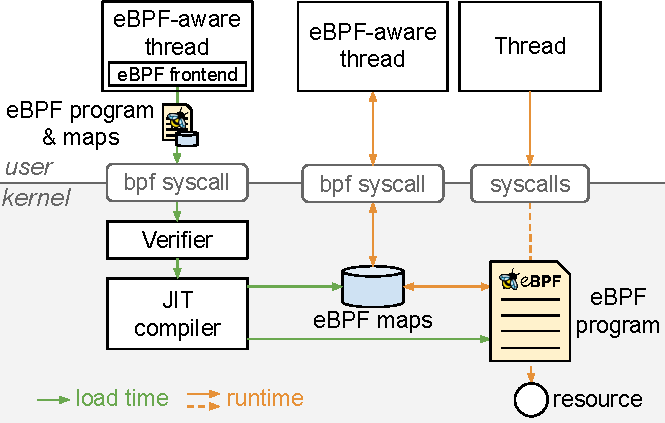
\includegraphics[width=0.9\columnwidth]{chapters/natisand/fig/bpf_bg}
  \caption{Overview of the eBPF architecture}
  \label{fig:bpf_sandbox}
\end{figure}

\subsubsection*{Seccomp}

Seccomp~\cite{seccompbpf} is a mechanism
provided by the Linux kernel to restrict the system calls
available to a userspace application. The rationale is that the
implementation of system calls may be affected by bugs or errors,
therefore reducing the kernel surface exposed to an unprivileged
application narrows the attack surface.

The initial implementation of Seccomp restricted the set of allowed
system calls only to {\tt exit}, {\tt sigreturn}, {\tt read} and {\tt
  write} (on previously opened file
descriptors)~\cite{edge2015seccomp}. The implementation was greatly
extended in 2012, and it now permits to intercept system calls and
determine whether each of them is safe to execute.
To this purpose a {\em filter} program written in the cBPF
dialect must be provided. Unfortunately, a classic program has only
access to the values of the arguments passed to the system calls
(e.g., configuration {\em flags}), and pointers cannot be dereferenced
to avoid TOCTOU issues~\cite{seccomp-toctou}.

%%% Local Variables:
%%% mode: latex
%%% TeX-master: "../main.tex"
%%% End:
